\documentclass{article}

\title{Numerical Integration: Computing Methods and Comparing Accuracy}
\author{Jaden Krause}
\date{October 5, 2026}
\usepackage{float}
\usepackage{graphicx}
\usepackage{amsmath}

\renewcommand{\topfraction}{0.9}         % Allow tables to take up 90% of the top of a page
\renewcommand{\bottomfraction}{0.8}      % Allow tables to take up 80% of the bottom of a page
\renewcommand{\textfraction}{0.05}       % Allow text to squeeze into spaces as small as 5% of a page
\renewcommand{\floatpagefraction}{0.95}  % Only give a table its own blank page if it takes up 95%+ of the area

\begin{document}
\maketitle

\section{Introduction}
One of the main focuses of calculus is evaluating integrals. When it comes to computing integrals analytically, 
and making accurate approximations, there are several important considerations. In this paper, I will compare 
different methods of numerical integration and I will evaluate their accuracy at different mesh sizes.

\section{The Problem}
In this evaluation, the function we will be using is
\[
    f(x) = \sin^2(x)e^{-x}
\]
Our limits of integration are $x \in [0, \pi]$. Below is the list of formulas we will be using to compute the integral analytically:
\subsubsection*{Composite Midpoint Rule}
\begin{equation}
\int_{a}^{b} f(x) \,dx = h \sum_{i=1}^{m} f(w_i) + \frac{(b-a)h^2}{24} f''(c)
\end{equation}
where $h = (b - a)/m$ and $c$ is between $a$ and $b$. The $w_i$ are the midpoints of the $m$
equal subintervals of $[a,b]$.
\subsubsection*{Composite Trapezoid Rule}
\begin{equation}
\int_{a}^{b} f(x) \, dx = \frac{h}{2} \left( y_0 + y_m + 2 \sum_{i=1}^{m-1} y_i \right) - \frac{(b-a)h^2}{12} f''(c)
\end{equation}
where $h = (b - a)/m$ and $c$ is between $a$ and $b$.
\subsection*{Composite Simpson's Rule}
\begin{equation}
\int_{a}^{b} f(x) \, dx = \frac{h}{3} \left[ y_0 + y_{2m} + 4 \sum_{i=1}^{m} y_{2i-1} + 2 \sum_{i=1}^{m-1} y_{2i} \right] - \frac{(b-a)h^4}{180} f^{(iv)}(c)
\end{equation}
where $c$ is between $a$ and $b$.
\subsection*{Gaussian Quadrature}
\begin{equation}
\int_{-1}^{1} f(x) \, dx \approx \sum_{i=1}^{n} c_i f(x_i)
\end{equation}
\begin{equation}
\text{where } c_i = \int_{-1}^{1} L_i(x) \, dx, \quad i = 1, \dots, n.
\end{equation}

\section{Results}
Using these formulas, I evaluated the approximations given by numerical integration at several different mesh 
resolutions (values of $h$). Smaller mesh resolutions correspond to greater accuracy. I calculated the error 
of these methods by comparing to the known analytical derivative of our function, $F(x) = -\frac{e^{-x}}{10}(2\sin{2x}-\cos{2x}+5)$. 
Finally, I graphed the relationship between the error of each approximation and the mesh size $h$. The graph will 
show us the convergence rates and how error decreases as $h$ decreases. The variables $n$ and $h$ are inversely related, as $n$ 
represents the number of subintervals, and $h$ represents the width of each subinterval. Thus, as $n$ increases, $h$ decreases.
\begin{table}[h]
\centering
\caption{Errors of each method at specified values of $n$}
\label{tab:method_errors}
\begin{tabular}{|c|c|c|c|c|c|}
\hline
$n$ & Midpoint & Trapezoidal & Simpson & Gauss-2pt & Gauss-3pt \\
\hline
4  & 2.7957e-03 & 3.1796e-03 & 1.4487e-02 & 5.3799e-04 & 2.1696e-06 \\
8  & 1.6815e-04 & 1.9193e-04 & 8.0396e-04 & 3.2117e-05 & 3.4659e-08 \\
16 & 1.0405e-05 & 1.1887e-05 & 4.8127e-05 & 1.9832e-06 & 5.4340e-10 \\
32 & 6.4865e-07 & 7.4125e-07 & 2.9741e-06 & 1.2357e-07 & 8.4968e-12 \\
64 & 4.0515e-08 & 4.6302e-08 & 1.8535e-07 & 7.7174e-09 & 1.3278e-13 \\
\hline
\end{tabular}
\end{table}

\begin{table}[h]
\centering
\caption{Estimated Observed Convergence Rates (Slopes)}
\label{tab:convergence_rates}
\begin{tabular}{|l|c|}
\hline
Method & Slope \\
\hline
Midpoint    & 4.02 \\
Trapezoidal & 4.02 \\
Simpson     & 4.06 \\
Gauss-2pt   & 4.02 \\
Gauss-3pt   & 5.99 \\
\hline
\end{tabular}
\end{table}
\begin{figure}[htbp]
    \centering
    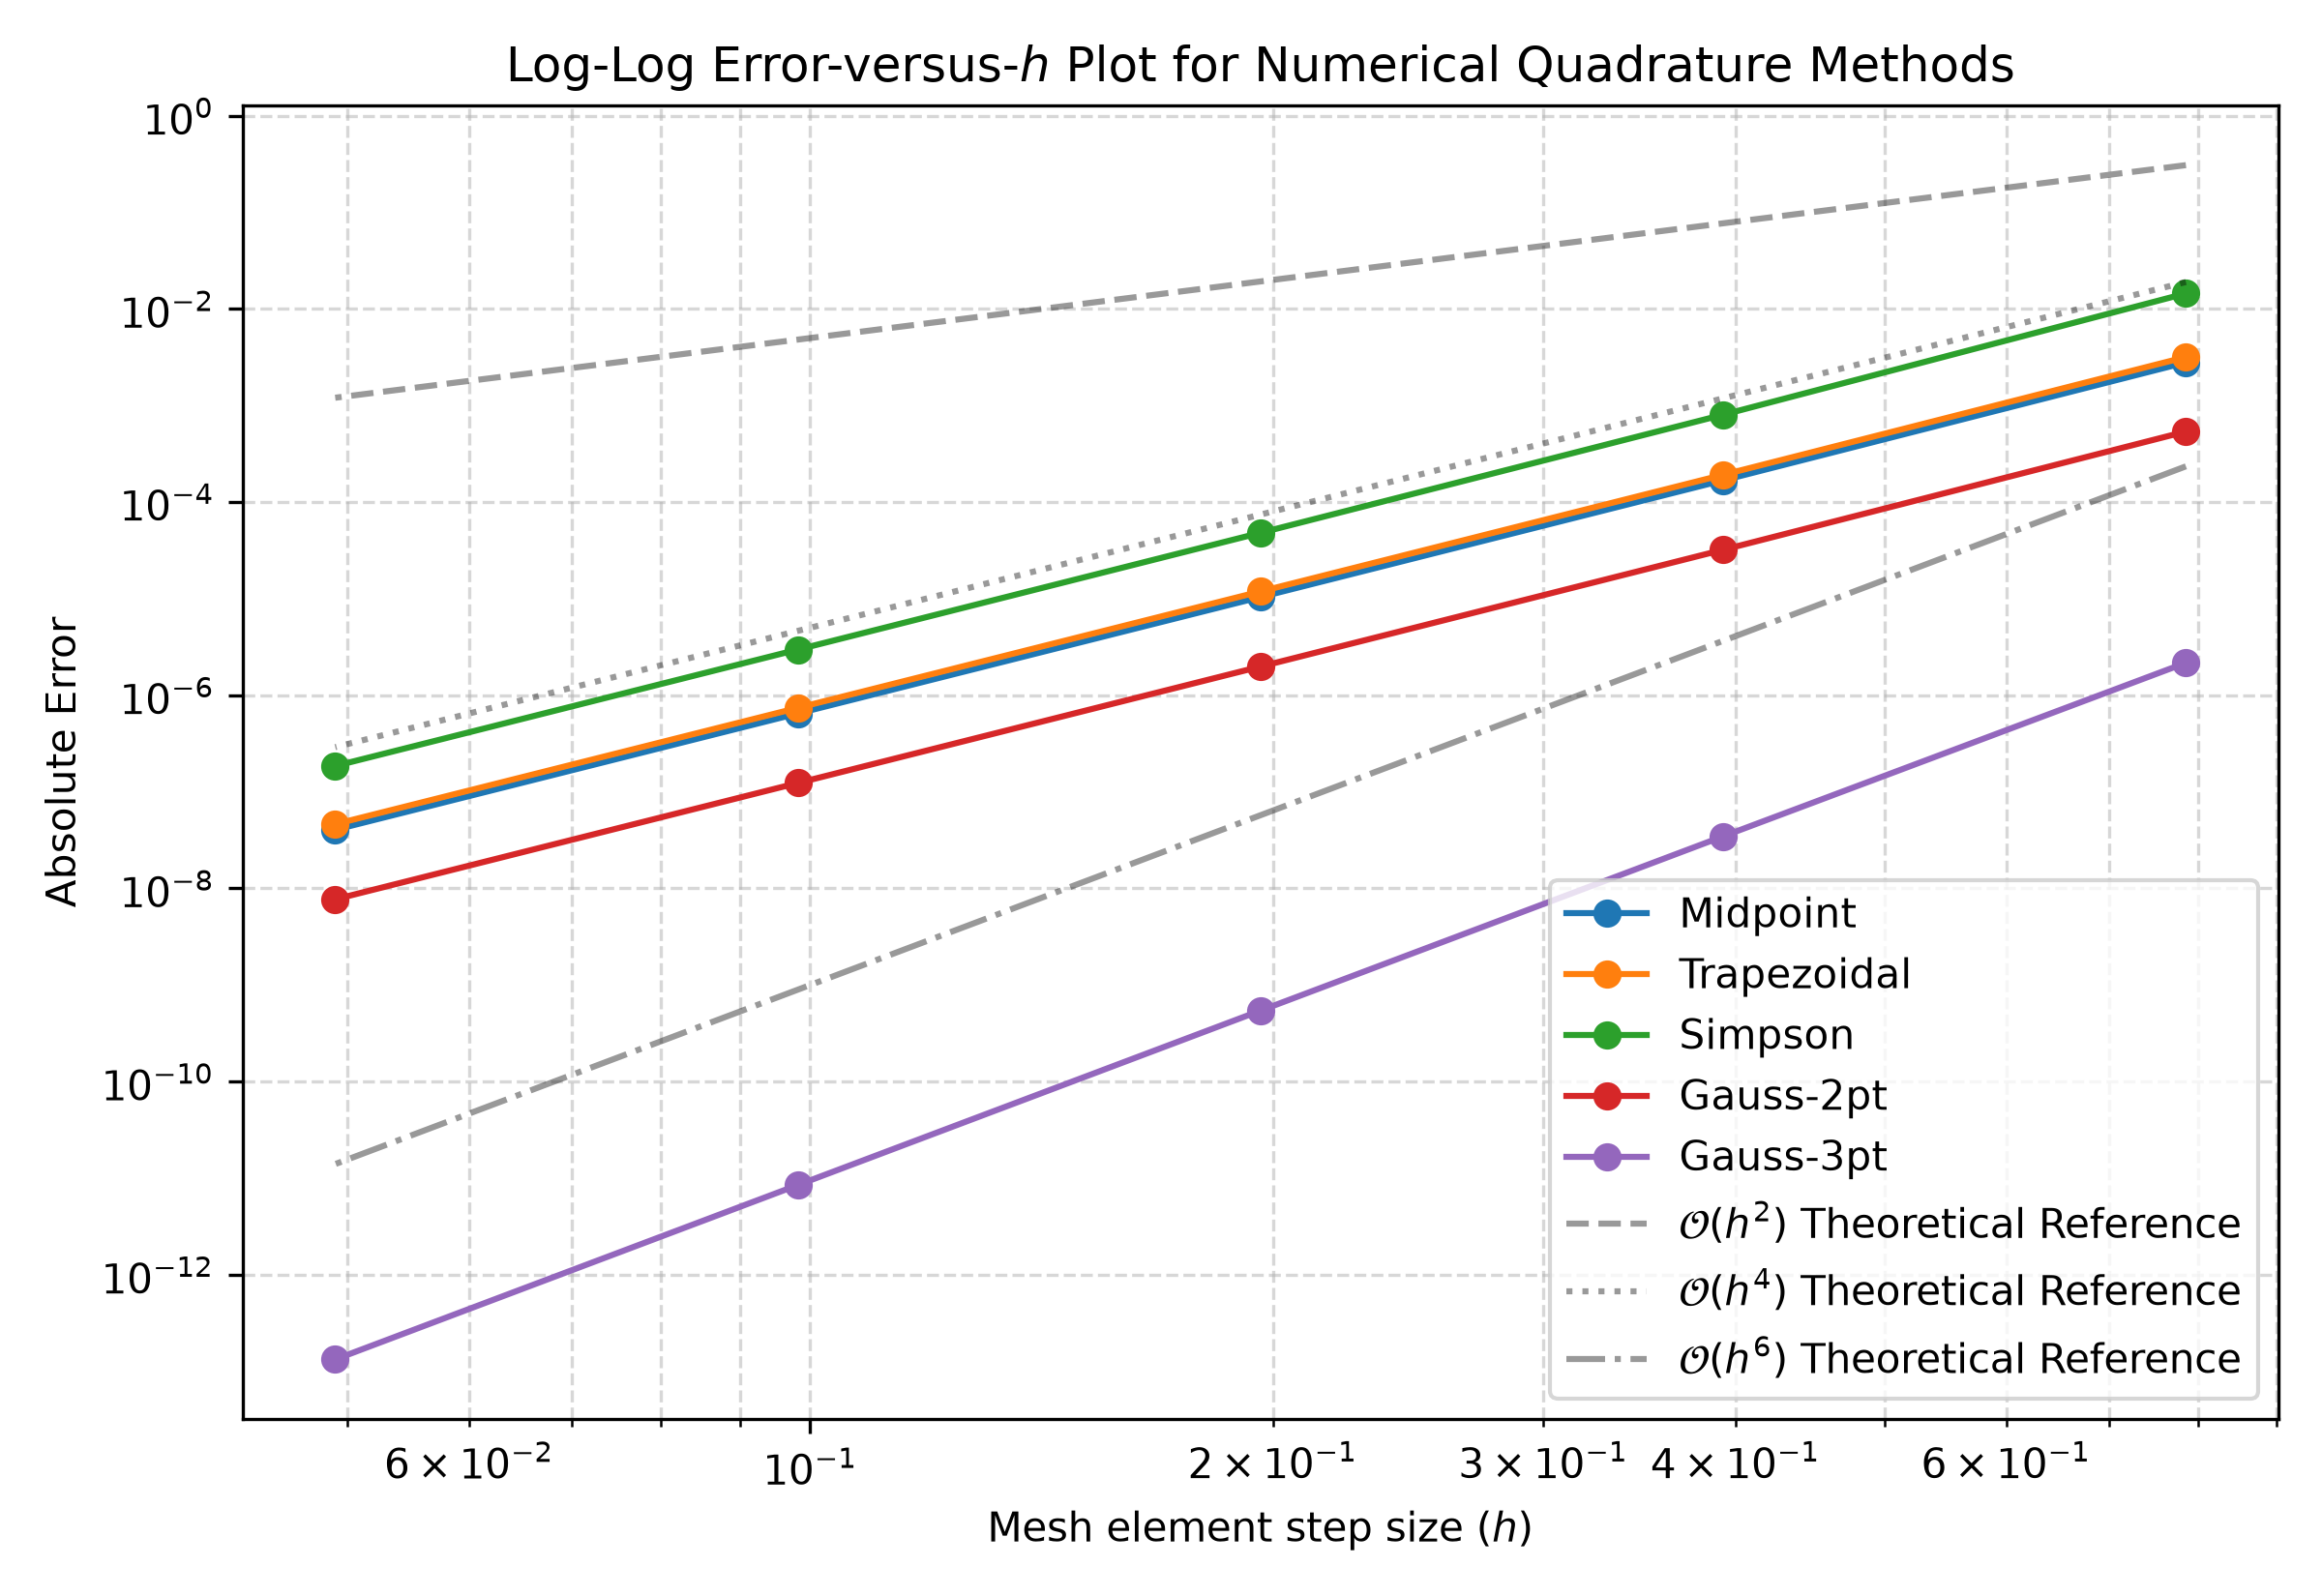
\includegraphics[width=1.0\textwidth]{quadrature_convergence_loglog.png}
    \caption{Error vs h}
\end{figure}
The convergence rates (slopes) in our graph agree with expectation. The deviation is in the Midpoint and Trapezoidal convergence lines.
The expected convergence rate for these methods is 2, and they show a convergence rate of 4, implying that they are more accurate 
than may be expected. This occurs because of the symmetry and periodic nature of our function, and that its value is 0 at both 
endpoints of the interval $x\in [0,\pi]$. This results in a cancellation of the error term in these functions, causing a phenomenon 
known as superconvergence and giving a more accurate result. 
\par
Otherwise, the other functions behave as expected. Simpson's Rule has a convergence rate of 4 and the 2-point Gaussian quadrature is 
the same. The 3-point Gaussian quadrature has a convergence rate of 6, corresponding to its higher accuracy.

\section{Conclusion}
In this paper, we compared the accuracy of several different methods of numerical integration. Each of them have their advantages, whether 
in their straightforward implementation or accuracy. 3-point Gaussian Quadrature yields the most accurate result compared to the rest 
of the methods we considered. However, with the relatively small errors each method produced, any of them could be used for the right problem.

\section{Bibliography}
Saur, Timothy (2017). \textit{Numerical Analysis}. 3rd es. Pearson ISBN: 9780134696454

\end{document}